\begin{frame}
	\frametitle{Satz von Ladner}
	\framesubtitle{Motivation}
	\includegraphics[page = 2,scale = 0.6]{images/npi.pdf}
	Frage : Gibt es $\NP$  Probleme, die nicht \NP -vollständig sind, aber auch
	nicht in $\P$  liegen?
\end{frame}
\begin{frame}
	\frametitle{Satz von Ladner}
	\framesubtitle{\NP -intermediate Probleme}
	Mögliche Kandidaten :
	\begin{itemize}
	\item Graphisomorphie (kommt in Vortrag 7)
	\item Faktorisierungsproblem
	\item Kein "natürliches" Problem bekannt
	\end{itemize}
	
	aber,
\end{frame}

\begin{frame}
	\frametitle{Satz von Ladner}
	\framesubtitle{Behauptung}
	\begin{KITinfoblock}{Existenz einer \NP -intermediate Sprache, Ladner, 75}
	Wenn $\P \neq \NP$ dann gilt : \newline
	Es existiert eine Sprache $L \in \NP \setminus \P$ die nicht \NP -vollständig ist
	\end{KITinfoblock}
\end{frame}
\begin{frame}
	\frametitle{Satz von Ladner}
	\framesubtitle{Beweisidee}
	Konstruieren Sprache mit diesen Eigenschaften und zeigen, dass sie in $\NP$ -
	intermediate ist, falls $\P \neq \NP$  :
	
	\bigskip
	\pause
	\begin{KITinfoblock}{Die Sprache ${\SAT}_H$}
		Für eine Funktion $H$ : $\mathbb{N} \rightarrow \mathbb{N}$ definieren wir : \newline 	
		${\SAT}_H = \lbrace \psi 01^{n^{H(n)}} : \psi \in \SAT$ und $ n = |\psi| \rbrace$
	\end{KITinfoblock}
	\bigskip
	\pause	
	
	\begin{KITexampleblock}{Beispiel für ${\SAT}_H$}
	F\"ur $H(n) = n - 1$ und $\psi = a \land b$ gilt : \newline
	$(a \land b) 01^{3^2} = (a \land b) 0111111111 \in {\SAT}_H $
	\end{KITexampleblock}
\end{frame}

\begin{frame}
	\frametitle{Satz von Ladner}
	\framesubtitle{Beweis : Wahl von $H$}
	\begin{KITinfoblock}{Definition von $H$}
		\begin{itemize}
		\item Betrachte die TM $M_1, M_2, ..., M_{\lfloor \log(\log(n)) \rfloor}$. \newline
		\item Wähle unter diesen die TM $M_i$ mit kleinster Gödelnummer $i$, welche für alle
		$|x| \leq \log(n) $  ${\SAT}_H(x)$
		in $i|x|^i$ Schritten berechnet
		\item Setze $H(n) = i$. 
		\item Falls eine solche TM nicht existiert, setze $H(n) = \log(\log(n))$
		\end{itemize}
	\end{KITinfoblock}
	\pause
	\begin{KITblock}{Gewähltes $H$ erfüllt die folgenden Eigenschaften}
		${\SAT}_H \in \P \Leftrightarrow H(n) \in O(1)$ (also $H(n) \leq C$ f\"ur alle n) 				\newline
		und damit insbesondere $\lim_{n \to \infty}  H(n) = \infty$ f\"ur ${\SAT}_H
		\notin \P$
	\end{KITblock}
	\pause
	\begin{itemize}
	  \item  $H$ erfüllt diese und ist polynomiell berechenbar.
	  \item (ohne Beweis)
	\end{itemize}
		
\end{frame}
% \begin{frame}{Beweis von Ladner}
% 	\framesubtitle{Nachweis der Eigenschaften von H}
%  	\begin{KITinfoblock}{Definition von H}
% 		$H(n)$ ist die kleinste Gödelnummer $i < \log (\log (n))$ so dass für alle
% 		$ x \in \{0,1\}^*$ mit $|x| \leq \log(n) $ die Turing Maschine $M_i$ genau ${\SAT}_H(x)$
% 		in $i|x|^i$ Schritten berechnet. Falls dieses $i$ nicht existiert setzen wir 
% 		$H(n) = \log(\log(n))$ 
% 	\end{KITinfoblock}
% 	\pause
% 	
% 	\begin{overprint}
% 		\only<2-5> {
% 			\bigskip
% 		Zuerst zeigen wir : ${\SAT}_H \in \P \Rightarrow H(n) \in O(1)$
% 		\pause
% 		\begin{itemize}[<+->]
% 			\item ${\SAT}_H \in \P \Rightarrow \exists$ Turing Maschine $M$, die
% 			${\SAT}_H$ in höchstens $cn^c$ Schritten entscheidet.
% 			\item $\exists i > c$ , so dass $M_i$ = M
% 			\item Für n > $2^{2^i}$ gilt $H(n) \leq i$ und damit $H(n) \in O(1)$ 
% 		\end{itemize}
% 		}
% 		\only<6-> {
% 			\bigskip
% 			Nun : $ H(n) \in \mathcal{O}(1) \Rightarrow {\SAT}_H \in \P$
% 			\pause
% 			\begin{itemize}
% 				\item<7-> Da $ H(n) \in \mathcal{O}(1)$ ist Bild von $H$ endlich $ \Rightarrow \exists i$ mit $H(n) = i$ für unendlich viele $n$
% 				\item<8-> TM $M_i$ löst ${SAT}_H$ in $ in^i$ Schritten
% 				\item<9-> Denn, angenommen $\exists x$ für welches $M_i$ dies nicht in dieser Grenze schafft $\Rightarrow$ $H(n) \neq i$ für alle $ n > 2^{|x|} $
% 				nach Definition von $H$
% 				
% 			\end{itemize}
% 		
% 		}
% 	\end{overprint}
% 	
% 	
% \end{frame}
\begin{frame}{Beweis von Ladner}
	\framesubtitle{${\SAT}_H$ weder in $\P$ noch  $\NP$-complete}
	\begin{KITinfoblock}{Definition von ${\SAT}_H$} 	
		${\SAT}_H = \lbrace \psi 01^{n^{H(n)}} : \psi \in \SAT$ und $ n = |\psi| \rbrace$
	\end{KITinfoblock}
	\begin{KITblock}{Gewähltes $H$ erfüllt die folgenden Eigenschaften}
			${\SAT}_H \in \P \Leftrightarrow H(n) \in O(1)$ (also $H(n) \leq C$ f\"ur alle n) 		
	\end{KITblock}
	\pause
	\bigskip
	\heading{${\SAT}_H$ ist nicht in $\P$}
	\pause
	\bigskip
	\begin{itemize}[<+->]
		\item Angenommen ${\SAT}_H \in \P \Rightarrow $  $H(n) \le C$, $C$ Konstante
		\item ${\SAT}_H$ ist also $\SAT$  mit höchsten polynomiell vielen  angehängten 1en
		\item $\SAT$ kann somit durch dieselbe TM wie ${\SAT}_H$ gelöst werden
			\begin{itemize}
				\item Konstruiere für Eingabe $\varphi$ die ${\SAT}_H$-Instanz $\varphi01^{|\varphi|^{H(|\varphi|)}}$ 
				\item gebe diese Instanz in TM, welche ${\SAT}_H$ polynomiell entscheidet
			\end{itemize}
			\item $\Rightarrow \P = \NP$
	\end{itemize}
	
\end{frame}

\begin{frame}{Beweis von Ladner}
		\framesubtitle{${\SAT}_H$ weder in $\P$ noch $\NP$-complete}
	
		\begin{KITinfoblock}{Definition von ${\SAT}_H$}	
			${\SAT}_H = \lbrace \psi 01^{n^{H(n)}} : \psi \in \SAT$ und $ n = |\psi| \rbrace$
		\end{KITinfoblock}
		
		
		\bigskip
		\only<2->{\heading{${\SAT}_H$ ist nicht in $\NPC$}}
		\pause
		\bigskip
		
		\begin{itemize}[<+->]
			\item Angenommen ${\SAT}_H \in \NPC \Rightarrow $ es existiert poly. Reduktion $f$ von $\SAT$ auf ${\SAT}_H$.
			\item Da ${\SAT}_H \notin \P $ geht $H(n)$ gegen $\infty$ 
			\item $\SAT$-Instanz $\varphi$ wird mit $f$ auf ${\SAT}_H$-Instanz der Form $\psi01^{{\psi}^{H(|\psi|)}}$ abgebildet.
			\item $|f(\varphi)|=|\psi| + |0| + {|\psi|}^{H(|\psi|)}$
		\end{itemize}
\end{frame}
\begin{frame}{Beweis von Ladner}
	\framesubtitle{${\SAT}_H$ weder in $\P$ noch $\NP$-complete}
	
	\begin{KITinfoblock}{Definition von ${\SAT}_H$}	
		${\SAT}_H = \lbrace \psi 01^{n^{H(n)}} : \psi \in \SAT$ und $ n = |\psi| \rbrace$
	\end{KITinfoblock}
		\begin{itemize}[<+->]
		\item Für beliebig große $\SAT$-Instanz $\varphi$ wird $|\psi|$ in ${\SAT}_H$ beliebig groß.
		\item $\Rightarrow$ ab gewisser Größe müssen $\SAT$-Instanz $\varphi$ von $f$ auf ${\SAT}_H$-Instanz mit $|\psi| \in o(n)$  abgebildet werden.
		 
		\item Ansonsten wegen $H(n)$ gegen $\infty$ \newline $|{|\psi|}^{H(|\psi|)}|$  und damit $ \Rightarrow|\psi01^{|\psi|^{H(|\psi|)}} |$  größer als jedes $p(|\varphi|)$.
		\item $|\psi|$ also echt kleiner als $\frac{|\varphi|}{2}$
		\item Algorithmus der $\SAT$ in poly. Zeit entscheidet 
			\begin{itemize}
				\item bilde $\SAT$-Instanz $\varphi$ mit $f$ auf $\psi01^{|\psi|^{H(|\psi|)}}$ ab
				\item $|\psi|$ kleiner $\frac{|\varphi|}{2}$ und es gilt $\varphi \in \SAT \Leftrightarrow \psi \in \SAT$ 
				\item Wiederhole ersten Schritt mit $\psi$ als Eingabe
			\end{itemize}
		\item Widerspruch zu $\P \neq \NP$
		\end{itemize}
\end{frame}